% Условная компиляция для самостоятельной работы
\ifdefined\mainfile
% Если это часть основного файла, не добавляем начало и конец документа
\else
\documentclass[12pt, a4paper]{report}
\usepackage{/Users/vladbelousov/Desktop/Semestr_4-FP-NSU/Настройка/library}
\usepackage[utf8]{inputenc} % Подключение поддержки UTF-8
\begin{document}
\fi

%%-------------------------------%%

\begin{definition}
     Углом между ненулевыми векторами x и y  евклидова пространства \( L  \)  называется число \( \varphi \in  [ 0, \pi ] \):

     \[ \cos \varphi = \frac{(x,y )}{\left\lVert x  \right\rVert \left\lVert y  \right\rVert}  \] 
\end{definition}

\begin{definition}
    Если S - подпространство пространства со скалярным произведением \( L \), то \( x \in  S  \)  называется вектором наилучшего приближения (ближайший) для \( y \in L      \)  посредством векторов из \( S  \), если: 

    \begin{center}
        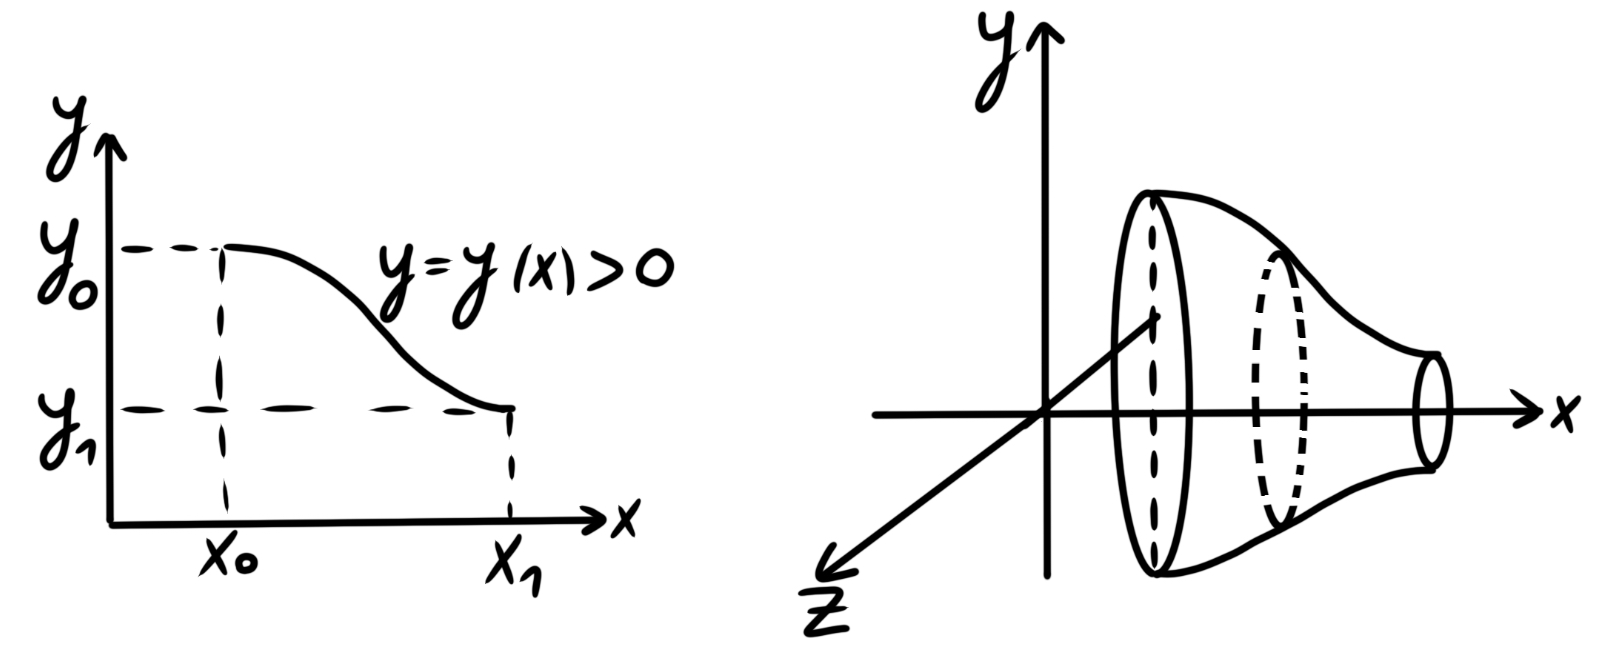
\includegraphics[width=0.3\textwidth]{/Users/vladbelousov/Desktop/Semestr_4-FP-NSU/ОФА/Лекции_по_дням/image/2.png}
    \end{center}

    \[ \forall z \in  S , \quad  \left\lVert y - z  \right\rVert \geq  \left\lVert x - y  \right\rVert \] 

    \[ \left\lVert x - y  \right\rVert  = \inf _{z \in  S } \left\lVert y -z  \right\rVert  \] 
\end{definition}

\begin{theorem}
    Пусть \( H  \)   - гильбертово пространство, \( S  \)   - замкнутое подпространство \( H , \text{  }  y \in  H  \), тогда \( \exists  ! x  \) ближайший к y.
\end{theorem}

\begin{proof}

    \[ \inf \left\lVert y -z  \right\rVert = d  \]  

    \[ x_1, \ldots, x_m \in  S \quad  \left\lVert  y - x_m       \right\rVert \xrightarrow{m \to  \infty } d   \] 

    \[ \left\lVert x_m - x_n         \right\rVert ^2 = \left\lVert (x_m - y ) - (x_n - y )  \right\rVert  ^2 = 2( \left\lVert  x_m - y   \right\rVert ^2 + \left\lVert  x_n - y      \right\rVert ^2 ) - \underset{_{\left\lVert x_m+ x_n - 2y  \right\rVert ^2 = 4 \left\lVert q - y  \right\rVert ^2 \geq 4 d ^2  }}{\left\lVert \underbrace{x_m - y + x_n - y }  \right\rVert }^2 \boxed{\le } \] 

    \[ q = \frac{x_m+ x_n }{2 } \in  S   \] 

    \[  \forall  \varepsilon , \exists  N \text{ }  n, m \geq  N :  \left\lVert x_m - y      \right\rVert  < d ^2 + \varepsilon \quad  \left\lVert  x_n - y  \right\rVert  ^2 \le  d ^2 + \varepsilon \] 

    \[ \boxed{\le  } 4 d ^2 + 2 \varepsilon - 4 d ^2 = 2 \varepsilon   \] 

    \[ x_m - \text{ фундаментальная }  \] 

    \[ \text{существование предела последовательности }   x: \] 

    \[  x \in  S , \text{ т.к }  S - \text{ замкнутое}  \] 

    \[ \left\lVert  y - x_n      \right\rVert = \sqrt{(y - x_n , y - x_n )} \underset{(1)}{\xrightarrow{n \to  \infty  } }\sqrt{(y - x, y -x )} = \left\lVert y -x  \right\rVert \to  d \text{ в силу ! предела}    \] 

    \begin{center}
        (1) - непрерывность по 1-му аргументу
    \end{center}

    Единственность: 

    \[ \text{Пусть } \tilde{x }: \left\lVert  y - \tilde{ x }\right\rVert = d , x \neq  \tilde{x } \] 

    \[ \left\lVert  \tilde{ x } - x      \right\rVert ^2 = \left\lVert  (\tilde{x }- y ) - ( x - y ) \right\rVert ^2 = 2\underset{= d ^2 }{\left\lVert \underbrace{\tilde{x }  - y}  \right\rVert}  ^2 +2\underset{= d ^2 }{\left\lVert \underbrace{x  - y}  \right\rVert} ^2 - \left\lVert 2 y - x - \tilde{x } \right\rVert ^2 \le 4 d ^2 - 4 d ^2 \le  0 \] 

    \[ \text{т.е } \tilde{x } = x - \text{ противоречие }  \] 

\end{proof}

\begin{definition}
    \( S  \)  - подпространство в линейном пространстве со скалярным произведением \( L, \text{ } x \in  S   \)  - ортогональная проекция \(  y \in  L   \)  на подпространство \( S  \), если: 

    \[ y- x \perp  S \quad  y -x \perp  z \text{ }  \forall  z \in  S \quad  ( y - x , z ) = 0  \] 

\end{definition}


\begin{lemma}
    \( S  \)  - подпространство в линейном пространстве со скалярным произведением \( L, \text{ }  x \in  S  \)  - ортогональная проекция \(  y \in  L  \Leftrightarrow   \)   x - ближайший к y посредством S.
\end{lemma}

\begin{proof}

    \[  \] 

    \( \boxed{\Rightarrow} :\) 
    
    \[ \forall  x, y , z \in  L \] 

    \[ \left\lVert  y - z  \right\rVert ^2  = ((y -x )+ (x- z ), (y -x) + ( x - z)) =   \] 
    
    \[ \overset{(1)}{=} \left\lVert y -x    \right\rVert ^2 + 2 \mathrm{Re }( \cancelto{0 }{x- y , x -z }) + \left\lVert x -z  \right\rVert ^2 (* ) \] 

    \[ (1): (a+b, a+ b )   = \left\lVert  a  \right\rVert ^2 + \left\lVert  b  \right\rVert ^2 + 2 \mathrm{Re } ( a,b ) \] 

    \[ x \in  S - \text{ ортогональная проекция y  на }  S \Rightarrow y -x \perp  x-z   \]  

    Итого: 

    \[ \left\lVert  y -z  \right\rVert ^2 = \left\lVert  y -x  \right\rVert ^2 + \underset{\geq 0 }{\left\lVert \underbrace{ x- z}  \right\rVert }^2  \] 

    \[ \forall  z \in  S : \left\lVert  y -z  \right\rVert ^2 \le  \left\lVert  y -x  \right\rVert ^2 , x - \text{ ближе для y }  \] 

    Пусть дано: 

    \( \boxed{\Leftarrow}: \) 

    \[ x - \text{ ближайший вектор для  } y \in S   \] 





    \[ \begin{aligned}
        \begin{array}{l|}
            \left\lvert y -x  \right\rvert = \inf \left\lVert  y -z \right\rVert \\
            f(t )  = \left\lVert  y -x + t W  \right\rVert ^2, \quad  t \in  \mathbb{R}  ^2 , \text{ }  W \in S
        \end{array}
        \Rightarrow f' (0 ) =0 
    \end{aligned} \] 

    \[ \lim_{t  \to 0}  \frac{ \left\lVert y -x + t W  \right\rVert ^2 - \left\lVert  y -x  \right\rVert ^2 } {t } = 0   \] 

    \[ \text{ в } (* ): z = x - t W  \]
    
    \[ \left\lVert y - (x - tW ) \right\rVert  ^2 - \left\lvert y -x  \right\rvert  ^2 = 2 \mathrm{Re } (y - x, t W ) + \left\lVert t W  \right\rVert ^2   \] 

    \[ \lim_{t  \to 0}    t\frac{2 \mathrm{Re } (y - x , W ) }{ t } + t ^2         \cancelto{0 }{ \frac{\left\lVert W  \right\rVert ^2 }{t } } = 0      \] 

    \[ 2 \mathrm{Re }  ( y - x, W )  = 0  \] 

    Если \( \mathrm{Im } ( y -x , W ) = 0 \), то x - ортогональная проекция y на S.

    Доказывается аналогично: \( f(t ) = \left\lVert y -x + i t W \right\rVert ^2 \)  

\end{proof}

\begin{definition}
    S - подпространство линейного пространства L  со скалярным произведением, то совокупность всех \( x \in  L    \), таких, что \( x \perp y \text{ }  \forall  y \in S  \) называется ортогональным дополнением к S  (\( S^{\perp }  \)).
\end{definition}

\begin{definition}
    Линейное пространство L является прямой суммой S  и T если любой вектор \( x \in  L      \)  единственным образом представим в виде \( x = y + z , \text{ }  y \in  S , \text{  } z \in  T  \) 
\end{definition}

\begin{lemma}
    H - гильбертово пространство, S - замкнутое подпространство, тогда H  прямая сумма S  и \(  S^{\perp } \) , \( H =   S \oplus S^{\perp }   \) 
\end{lemma}

\begin{proof}
    
    \[  y \in  H \quad  x - \text{ ближайший к y посредством S } \Rightarrow  \] 

    \[ \overset{\text{Лемма 1} }{\Rightarrow} y -x \perp  z , \text{ }  z \in  S \Rightarrow  \] 

    \[\Rightarrow  W = y -x \in  S^{\perp }  \]  

    \[ y = \overset{ \in  S ^{\perp } }{W} +\overset{\in  S }{ x}  \] 

    Докажем единственность представления: 

    Пусть \( y = \overset{ \in  S ^{\perp } }{\tilde{W }} + \overset{ \in  S ^{\perp } }{\tilde{ x }}  \) 

    \[  W + x = \tilde{ W } +\tilde{ x } \] 

    \[ W - \tilde{W } = \tilde{ x } - x  \] 

    \[ (\underset{\in  S ^{\perp }}{W- \tilde{W }}  , \underset{\in S}{ \tilde{ x } - x }) = (\tilde{x } -x , \tilde{x } - x ) \] 

    \[ 0 =  (\tilde{x } -x , \tilde{x } - x )\] 

    То есть: \( \tilde{x } = x  \text{ и }  \tilde{W } = W  \) 
\end{proof}

\begin{theorem}
    S - конечномерное подпространство линейного пространства L со скалярным произведением \( x_1, \ldots, x_n    \)  - ортонормированный базис в S \( \text{ } \forall  y \in  L     \):

    \[ x = \sum_{1} ^n \lambda_k x_k , \quad  \lambda_k = (y , x_k) \] 

    является ортогональной проекцией y на подпространство S. При этом: 

    \[  \left\lVert  y  \right\rVert ^2 =\left\lVert  x  \right\rVert ^2 + \left\lVert  y -x   \right\rVert ^2  \] 
\end{theorem}


\begin{proof}
    \[ \forall  z \in  S , \text{ }  z = \sum_{1} ^ n \alpha_k x_k  \] 

    \[  (z, x_m ) = \sum  _1 ^1 \alpha_k (x_k , x_m ) = \alpha_m \] 

    \[ \left\lVert z  \right\rVert ^2 = \left(  \sum  _ 1 ^ n \alpha_k x_k ,  \sum  _ 1 ^ n \alpha_p x_p  \right)  = \sum  _ 1 ^ n \alpha_p \left( \overline{\sum_1 ^ n \alpha_k x_k , x_p  }  \right) =\sum  _1 ^ n \alpha_p \left[ \sum  _1 ^ n \overline{\alpha_k } (\overline{x_p, x_k}  )   \right] =  \sum  _{k =1 }  ^{ n} \left\lvert  \alpha_k     \right\rvert  ^2 \]  

    \[ \left\lVert y -z  \right\rVert ^2 = \left\lVert y   \right\rVert ^2 - ( z, y ) -  ( y , z ) + \left\lVert z   \right\rVert ^2 = \left\lVert y  \right\rVert ^2 - \sum   _ 1 ^ n \alpha_k(x_k, y ) - \sum_{ 1} ^ n \overline{\alpha_k} (y, x_k ) +\sum_{ 1} ^n \left\lvert \alpha_k   \right\rvert ^2  = \]

    \[ =\left\lVert y  \right\rVert ^2 - \sum_{ 1 } ^ n \alpha_k \lambda_k - \sum_{ 1 } ^ n \overline{\alpha_k }\lambda_k +\sum_{ 1 } ^ n \left\lvert \alpha_k   \right\rvert ^2 +  \sum_{ 1 } ^ n \left\lvert \lambda_k      \right\rvert ^2- \sum_{ 1 } ^ n \left\lvert \lambda_k      \right\rvert ^2 = \left\lVert  y  \right\rVert ^2 + \sum_{ 1 } ^ n \left\lvert  \alpha_k - \lambda_k \right\rvert ^2  -\sum_{ 1 } ^ n \left\lvert \lambda_k     \right\rvert ^2       \] 

    \[ \left\lVert y  \right\rVert ^2 - \sum_{ 1 } ^ n \left\lvert \lambda_k     \right\rvert ^2 \geq 0  , \text{ при }  \alpha_k = \lambda_k \text{ } (z = x )  \] 

    При z = x  достигается минимум \( \Rightarrow   \)  ортогональная проекция.

\end{proof}

\begin{definition}
    \( x_1, \ldots, x_n, \ldots,  \)  - ортонормированная система в линейном пространстве со скалярным пространством L: 

    \[ x \in  L \quad  \lambda_k = ( x , x_k ) - \text{ коэффициент Фурье x.}  \] 

    \[ \sum_{ n= 1 } ^{\infty } \lambda_k x_k - \text{ ряд Фурье расходится}  \] 


\end{definition}

\begin{theorem}[неравенстов Бесселя]    
    \( x \in  L  \)  - линейное пространство со скалярным произведением, \( \lambda_k  \)  - коэффициент Фурье, тогда:

    \[ \sum_{k =1}^{\infty  } \left\lvert  \lambda_k     \right\rvert ^2 \le  \left\lVert x  \right\rVert ^2  \] 


\end{theorem}

\begin{proof}
    \[ <x_1, \ldots, x_n> \] 

    \[ S_n = \sum_{k =1}^{n  }   \lambda_k x_k\] 

    \[\underbrace{ \left\lVert x - S_n   \right\rVert}_{> 0} ^2   + \left\lVert S_n      \right\rVert ^2 = \left\lVert x  \right\rVert ^2 \] 

    \[ \left\lVert  S_n      \right\rVert  ^2 \le  \left\lVert x  \right\rVert ^2 \] 

    \[ \left( \sum_{k=1} ^{n  } \lambda_k x_k , \sum_{k=1} ^{n  } \lambda_k x_k  \right) \le  \left\lVert x  \right\rVert ^2 \] 

    \[ \sum_{k=1} ^{n  } \left\lvert \lambda_k     \right\rvert ^2 \le  \left\lVert x  \right\rVert ^2 \] 

    \[ \sum_{k=1} ^{n  } \left\lvert \lambda_k     \right\rvert ^2 \le  \left\lVert x  \right\rVert ^2 \] 
    \[ \overset{\displaystyle \downarrow }{\text{ в пределе}}  \]

    \[ \sum_{k=1} ^{\infty  } \left\lvert \lambda_k     \right\rvert ^2 \le  \left\lVert x  \right\rVert ^2   - \text{ равенство Парсеваля}  \] 

\end{proof}



%%-------------------------------%%

% Закрытие документа, если файл компилируется отдельно
\ifdefined\mainfile
% Если это основной файл, не нужно заканчивать документ
\else
\end{document}
\fi